\Question{Fisher's Linear Discriminant Analysis}
\textit{(Inspired by section 4.3.3 of ESL.)}

Suppose we have a binary classification problem for which we would like to find a linear estimator for--that is,
given a random vector $\vec{X}$, we would like to find predictor $Z = w^\top \vec{X}$, s.t. we maximize $(E[Z|Y=1] - E[Z|Y=0])^2$.\\

We define:\\
$\mu_i = E[X|Y=i]$\\
$\Sigma = (\vec{X}-\mu_i)(\vec{X}-\mu_i)^\top$, where for both classes $i=0,1$ we have the same covariance matrix.\\
$n_0 = n_1$, i.e. the number of data points in each class are the same.\\

Thus we have
\begin{align*}
\begin{aligned}
\max (E[Z|Y=1] - E[Z|Y=0])^2 &= \max (E[w^\top \vec{X}|Y=1] - E[w^\top \vec{X}|Y=0])^2 \\
&= \max (w^\top (E[\vec{X}|Y=1] - E[\vec{X}|Y=0]))^2 \\
&= \max (w^\top (\mu_1 - \mu_0))^2\\
&= \max w^\top (\mu_1 - \mu_0)(\mu_1 - \mu_0)^\top w
\end{aligned}
\end{align*}

\begin{Parts}

\Part Given the above maximization problem, we know that $|w|$ can increase without bound unless we have some kind of normalization.
One way we can normalize is to divide by the magnitude of $w$. What is the result of this normalization?

\begin{solution}
Normalizing as instructed, we have:
$$\max {w^\top (\mu_1 - \mu_0)(\mu_1 - \mu_0)^\top w \over w^\top w}$$

Note that while this looks similar to the Rayleigh quotient, this is not PCA, since $(\mu_1 - \mu_0)(\mu_1 - \mu_0)^\top$ has a rank of 1.

\end{solution}

\Part Is the approach from part (a) equivalent to LDA?
Refer to this plot from ESL to explain your conceptual answer. The crosses represent centroids. The ellipses represent an isocontour of the multivariate gaussian corresponding to the covariance matrix of a set of data.
The dotted line represents the decision boundary. The bell curves represent a projection of the multivariate gaussians.

\begin{center}
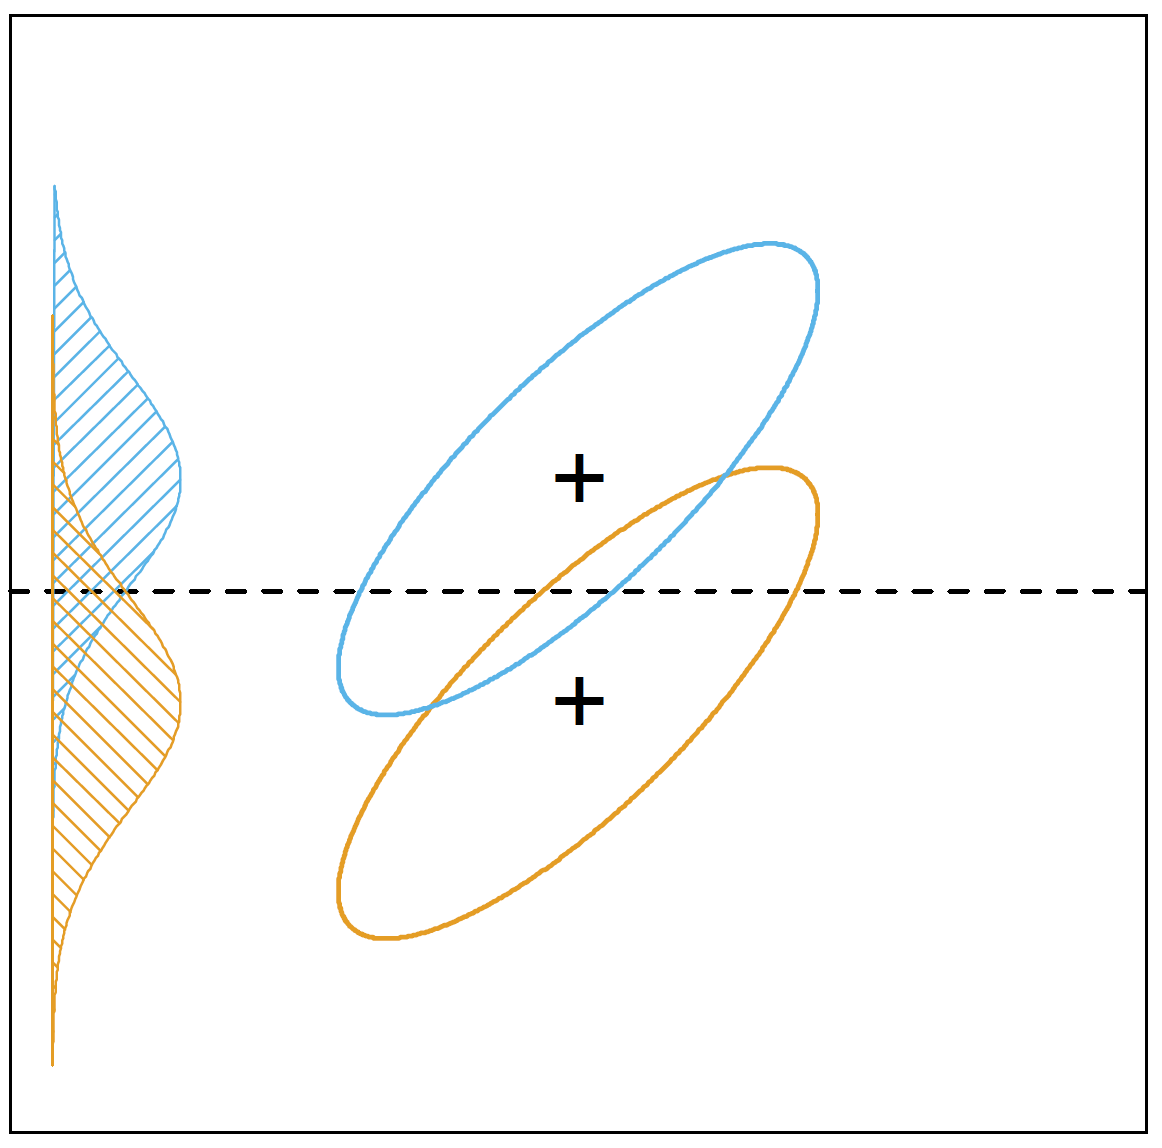
\includegraphics[width=2in]{src/problems/qda_lda/esl_lda_1.png}
\end{center}

\begin{solution}
No. This approach does not take into account the covariance matrices of the centroids whatsoever.
From the plot, we can see that under LDA, the decision boundary should not be the line that is simply equidistant to the two centroids.
\end{solution}

\Part Now, we will try normalizing instead by $\frac{1}{2}\text{var}[Z|Y=1]+\frac{1}{2}\text{var}[Z|Y=0]$.
Simplify in terms of $\Sigma$ and $\mu_i$ (refer to the definitions at the beginning of this problem).

\begin{solution}
\begin{align*}
\begin{aligned}
\frac{1}{2}\text{var}[Z|Y=1]+\frac{1}{2}\text{var}[Z|Y=0] &= \text{var}[w^\top \vec{X} | Y] \\
&= E[w^\top(\vec{X}-\mu_i) | Y]^2 \\
&= w^\top(\vec{X}-\mu_i)(\vec{X}-\mu_i)^\top w \\
&= w^\top \Sigma w
\end{aligned}
\end{align*}

Thus we have,
$$\max {w^\top (\mu_1 - \mu_0)(\mu_1 - \mu_0)^\top w \over w^\top \Sigma w}$$
\end{solution}

\Part Prove that your approach from part (c) is indeed equivalent to the decision boundary of LDA you are familiar with by
finding $w$ s.t. $w^\top x = c$, for some constant $c$.
(Take it that solving for $w$ through Lagrange multipliers yields that $w \propto \Sigma^{-1} (\mu_1-\mu_0)$.)

$(x-\mu_0)^\top \Sigma(x-\mu_0) = (x-\mu_1)^\top \Sigma(x-\mu_1) = \dots$

\begin{solution}
\begin{align*}
\begin{aligned}
(x-\mu_0)^\top \Sigma^{-1}(x-\mu_0) &= (x-\mu_1)^\top \Sigma^{-1}(x-\mu_1) \\
x^\top \Sigma^{-1} x - \mu_0^\top \Sigma^{-1} x - x^\top \Sigma^{-1} \mu_0 + \mu_0^\top \Sigma^{-1} \mu_0 &= x^\top \Sigma^{-1} x - \mu_1^\top \Sigma^{-1} x - x^\top \Sigma^{-1} \mu_1 + \mu_1^\top \Sigma^{-1} \mu_1\\
- 2\mu_0^\top \Sigma^{-1} x  + \mu_0^\top \Sigma^{-1} \mu_0 &= - 2\mu_1^\top \Sigma^{-1} x + \mu_1^\top \Sigma^{-1} \mu_1\\
2\mu_1^\top \Sigma^{-1} x- 2\mu_0^\top \Sigma^{-1} x  &=  c\\
\mu_1^\top \Sigma^{-1} x- \mu_0^\top \Sigma^{-1} x  &=  c\\
(\mu_1-\mu_0)^\top \Sigma^{-1} &\propto w^\top \\
w &\propto \Sigma^{-1}(\mu_1-\mu_0)
\end{aligned}
\end{align*}
Since we found that $w$ is equivalent to what Lagrange multipliers yields, as given to us, we can conclude that these formulations are equivalent.
\end{solution}

\Part Interpret why the approach from parts (c) and (d) are conceptually equivalent to LDA?
Refer to this plot from ESL to explain your answer.

\begin{center}
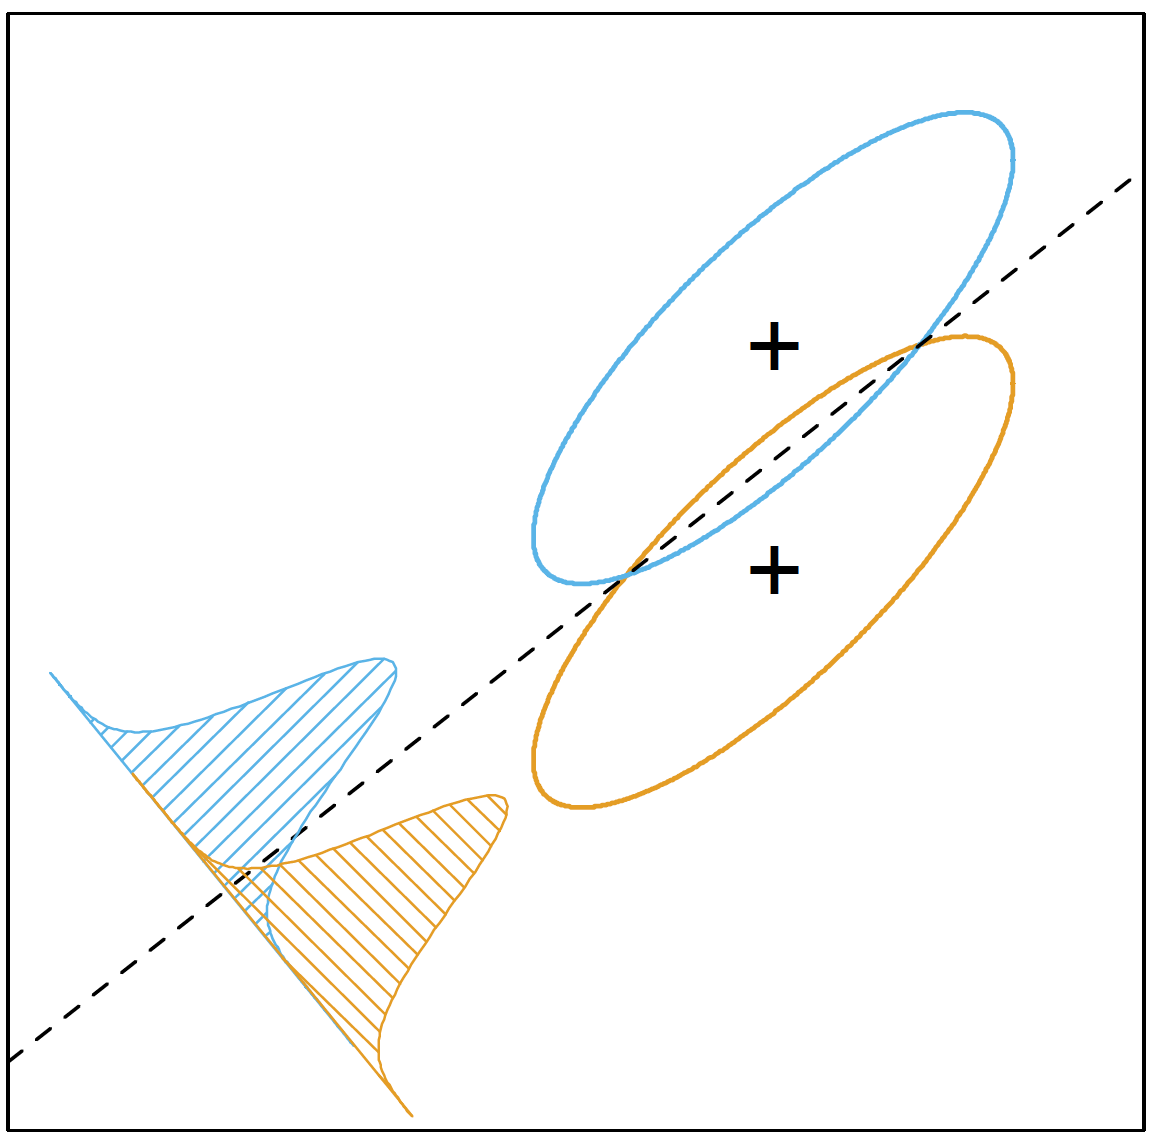
\includegraphics[width=2in]{src/problems/qda_lda/esl_lda_2.png}
\end{center}

\begin{solution}
Yes. $w$ is the axis along which these projected distributions have minimal intersection.
This is equivalent to maximizing the variance of the projection of the centroids (i.e. the means of the projected distributions), divided by the projected variance of the distributions themselves.
\end{solution}

\end{Parts}
